\documentclass{article}
\usepackage[utf8]{inputenc}
\usepackage{graphicx}

\title{Tugas Besar Database II (Membuat Aplikasi Di Orecle APEX)}

\author{Dyah Ayu Anandra}
\date{1184098}

\begin{document}

\maketitle

\section{Pengertian APEX}
\hspace \paragraph{Oracle Application Express atau APEX sebelumnya bernama Oracle HTML DB, merupakan pengembangan perangkat lunak berbasis web yang berjalan pada database Oracle. Dan sepenuhnya didukung dan dilengkapi standar tanpa biaya tambahan dengan semua edisi Oracle Database, diinstal secara standar sebagai bagian dari instalasi basis data inti. APEX dapat digunakan untuk membangun sebuah aplikasi web yang kompleks yang dapat digunakan di sebagian besar browser web modern. Lingkungan pengembangan APEX juga berbasis browser.Tujuan dibuat Apex supaya bisa mengembangkan Aplikasi Web atau Mobile Secara Cepat di lingkungan Oracle.}
\hspace \paragraph{APEX dibuat oleh Mike Hichwa, seorang pengembang di Oracle, setelah pengembangan proyek sebelumnya, Web DB, mulai menyimpang dari visi aslinya. Meskipun APEX berbagi beberapa fungsionalitas dengan Web DB, itu dikembangkan dari awal dan tidak ada jalur peningkatan dari Web DB ke APEX. Ketika ditugaskan membangun kalender web internal, Hichwa meminta bantuan Joel Kallman dan memulai pengembangan proyek yang disebut Arus. Hichwa dan Kallman bersama-sama mengembangkan Kalender dan Alur Web, menambahkan fitur ke Aliran karena mereka membutuhkannya untuk mengembangkan kalender. Build awal Flow tidak memiliki front-end sehingga semua perubahan pada aplikasi harus dibuat dalam SQL * Plus melalui sisipan, pembaruan, dan penghapusan.}

\hspace \paragraph{Application Express atau APEX memiliki dua macam yaitu, APEX offline dan APEX online. Jika kita ingin memakai oracle APEX online maka kita dapat langsung mengakases di web browser, namun jika kita ingin memakai oracle offline maka kita harus menginstall oracle APEXnya terlebih dahulu. Untuk memasang oracle APEX offline di perangkat kita, pertama kita perlu mengunduh nya di web browser. Namun keduanya oracle APEX online ataupun offline kita perlu registrasi agar dapat login dan masuk ke halaman utama. Gambar di bawah ini merupakan tampilan login.}

\begin{center}
    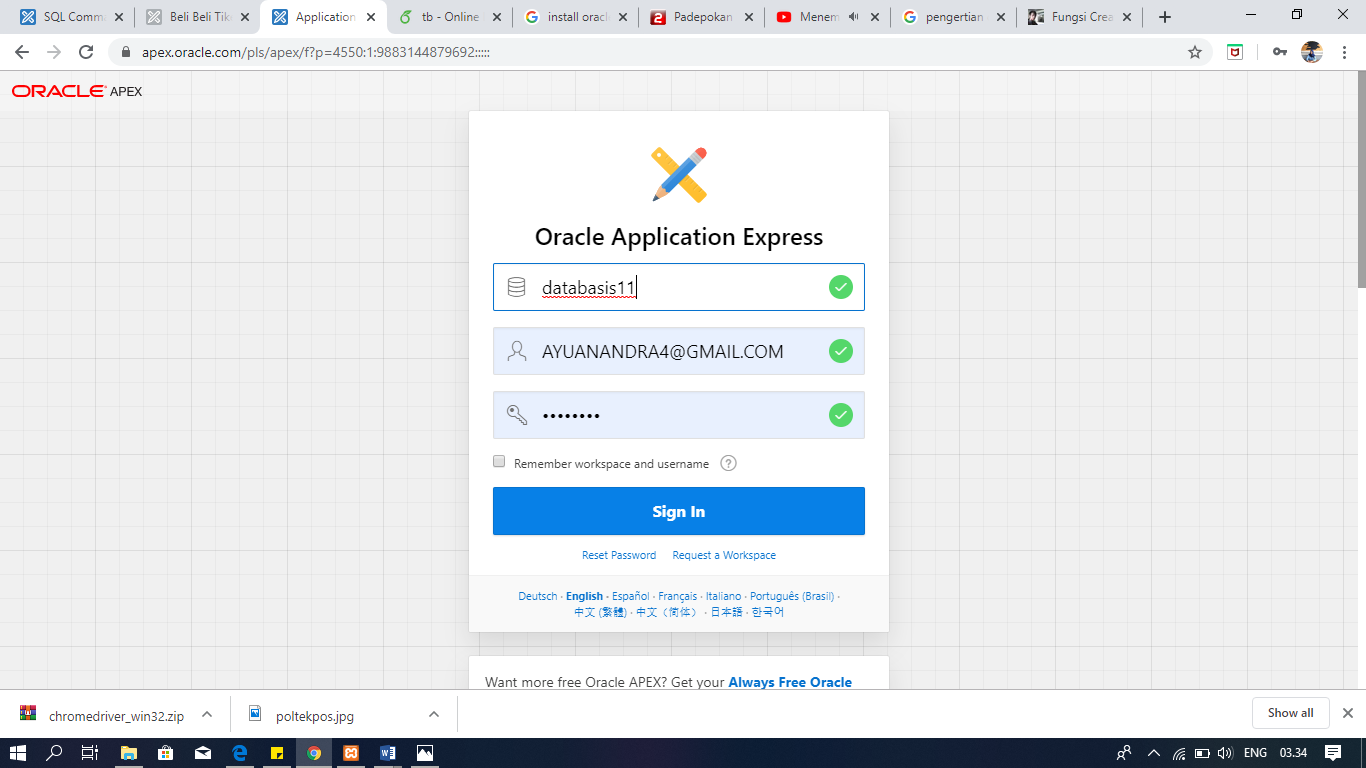
\includegraphics[width=10cm]{log.png}
\end{center} ||

\begin{center}
    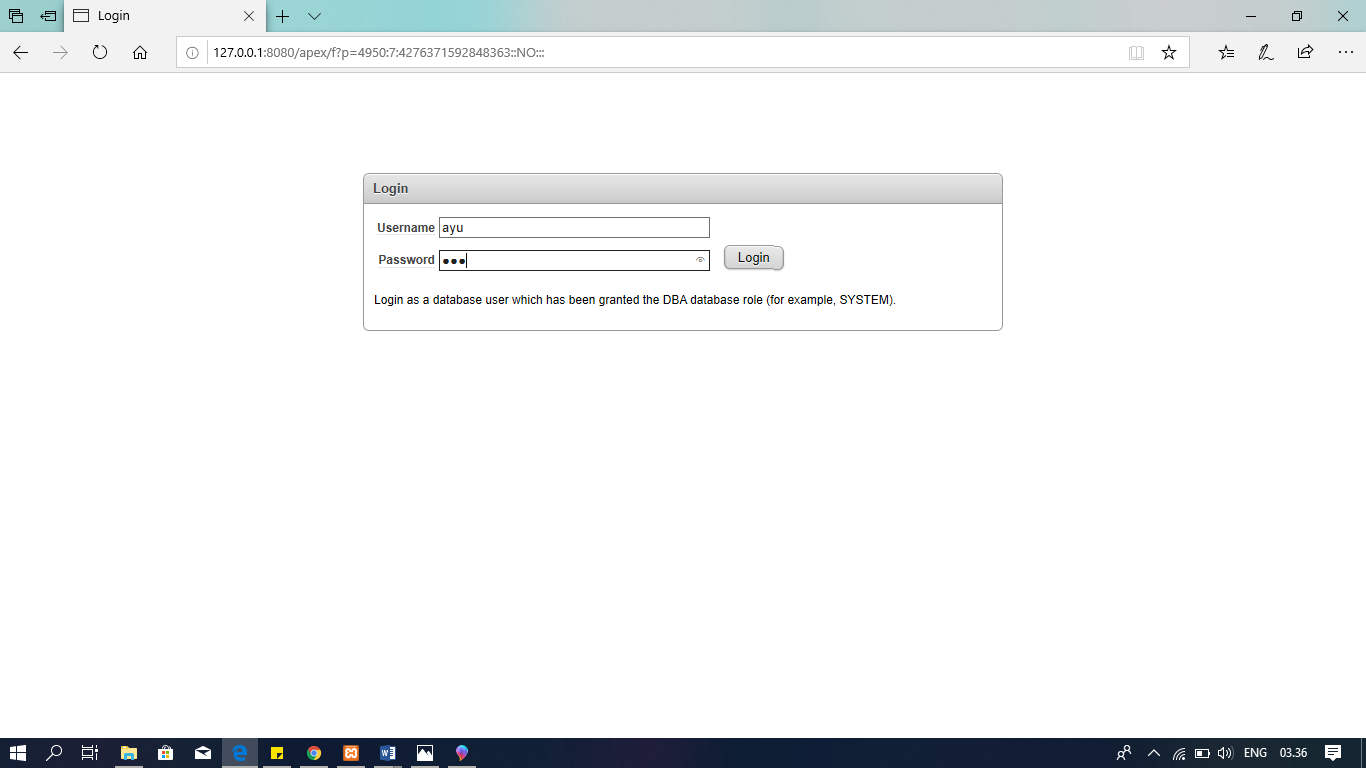
\includegraphics[width=10cm]{in.png}
\end{center}

\section{Aplikasi Beli Beli Tiket Dot Com}
\hspace \paragraph{Aplikasi beli beli tiket dot com merupakan sebuah aplikasi untuk memesan tiket pesawat saja, di dalam nya ada tiga table yaitu, table konsumen, table pembayaran, dan table tiket. Dan aplikasi ini dibuat menggunakan oracle APEX online.}  

\section{Persiapan Sebelum Membuat Aplikasi Di Oracle APEX}
\begin{enumerate}
    \item Login ke Oracle APEX terlebih dahulu, dapat memakai oracle APEX yang online atau offline.
    \item Klik SQL Workshop dan pilih SQl Commands untuk menuliskan query yang akan kita buat, pertama kita akan membuat table dan di Aplikasi beli beli tiket pesawat dot com ini memiliki tiga table yaitu, table konsumen, table pembayaran, dan table tiket.
    Create table adalah Pernyataan ini digunakan untuk menciptakan suatu tabel dalam basis data.
    \item ketikan query untuk membuat table pertama table Konsumen, di dalam table konsumen ini ada kolom, no identitas, nama konsumen, alamat konsumen, no telephone, dan jenis kelamanin.  
    \begin{center}
    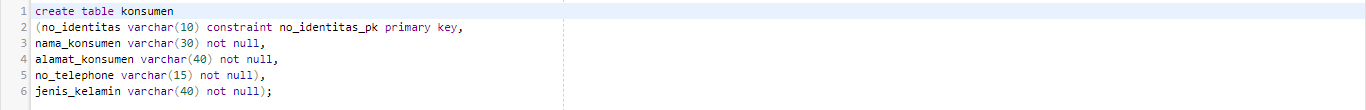
\includegraphics[width=10cm]{create konsumen.png}
    \end{center}
    \item ketikan query untuk membuat table kedua table pembayaran, di dalam table pembayaran ini ada kolom, no pembayaran, no tiket, tgl pembayaran, hari pembayaran, jumlah tiket, harga tiket, dan total pembayaran. 
    \begin{center}
    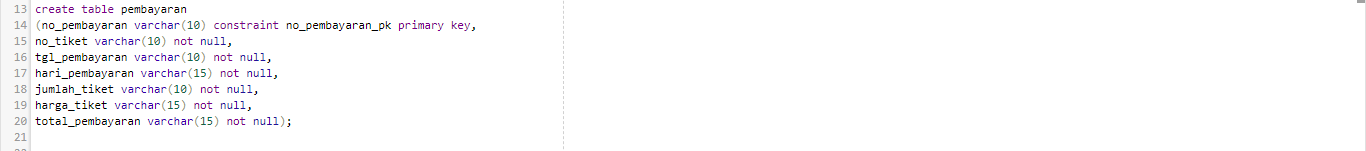
\includegraphics[width=10cm]{create pembayaran.png}
    \end{center}
    \item ketikan query untuk membuat table ketiga table tiket, di dalam table tiket ini ada kolom, no tiket, no kunsumen, tgl berangkat, hari berangkat, waktu berangkat.
    \begin{center}
    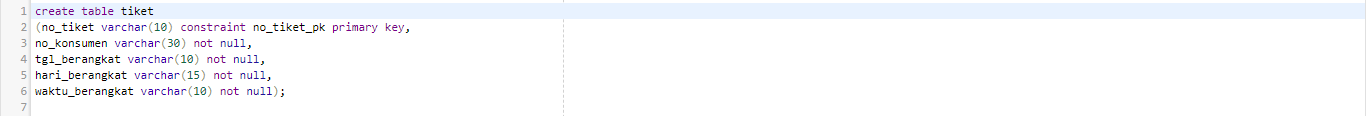
\includegraphics[width=10cm]{create tiket.png}
    \end{center}
    Insert adalah perintah untuk mengisi data baru dalam suatu tabel.
    \item Setelah semua table sudah dibuat, Tabel yang akan kita isi data adalah tabel konsumen yang kolomnya terdiri dari: '002','Anandra','Sariasih','082278702211','Perempuan', '003','Annisa','Sarijadi','082321871543','Perempuan', 
    '004','Almi','Sarimanah','082326512829','Laki-Laki';
    \begin{center}
    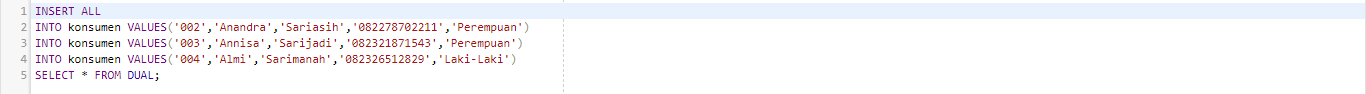
\includegraphics[width=10cm]{insert konsumen.png}
    \end{center}
    \item Tabel kedua yang akan kita isi data adalah tabel pembayaran yang kolomnya terdiri dari: 
    '098','123','11-02-2020','Senin','1','200000','200000',
    '100','135',15-03-2020','Rabu','1','400000','400000',
    '150','142','22-12-2020','Kamis,'1','500000','500000';
    \begin{center}
    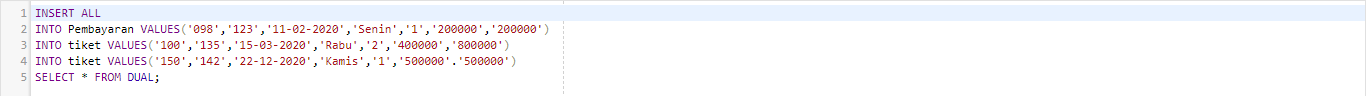
\includegraphics[width=10cm]{insert pembayran.png}
    \end{center}
    \item Tabel ketiga yang akan kita isi data adalah tabel tiket yang kolomnya terdiri dari: 
    '123','002','11-02-2020','Senin','10.10',
    '135','003','15-03-2020','Rabu','12.00',
    '142,'004','22-12-2020','Kamis','14.00';
    \begin{center}
    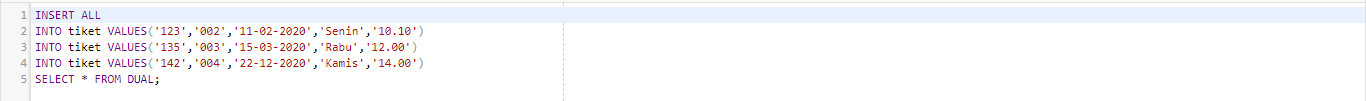
\includegraphics[width=10cm]{insert tiket.png}
    \end{center}
    \item buatlah table history dari table pembayaran (tergantung dengan table yang akan kita jadikan trigger) gunanya table ini adalah untuk memanggil table di trigger.
    Trigger basis data adalah prosedur tersimpan khusus yang dijalankan ketika tindakan tertentu terjadi dalam basis data. Sebagian besar trigger didefinisikan untuk dijalankan ketika perubahan dilakukan pada data tabel. Trigger juga dapat didefinisikan untuk menjalankan perintah sebelum atau setelah eksekusi DML (Data Manipulation Language) seperti INSERT, UPDATE, dan DELETE. Trigger banyak digunakan untuk menjaga integritas informasi pada database. Contohnya seperti di bawah ini. Pada aplikasi ini untuk trigger nya terdapat ditable pembayaran.
    \item Ketikan query trigger Delete pada table pembayaran
     \begin{center}
    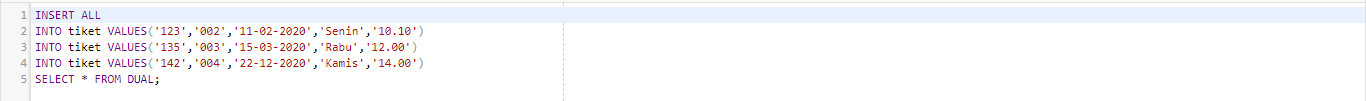
\includegraphics[width=10cm]{insert tiket.png}
    \end{center}
    \item Ketikan query trigger Update pada table pembayaran
     \begin{center}
    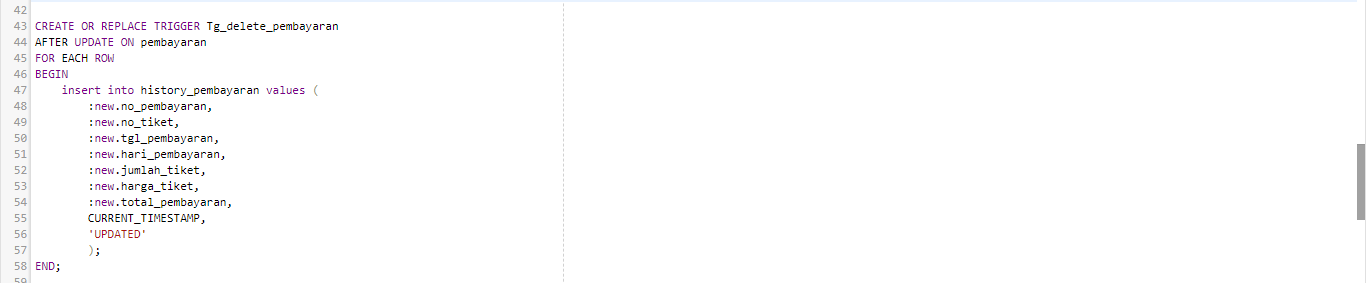
\includegraphics[width=10cm]{update.png}
    \end{center}
    \item Ketikan query trigger Insert pada table pembayaran
     \begin{center}
    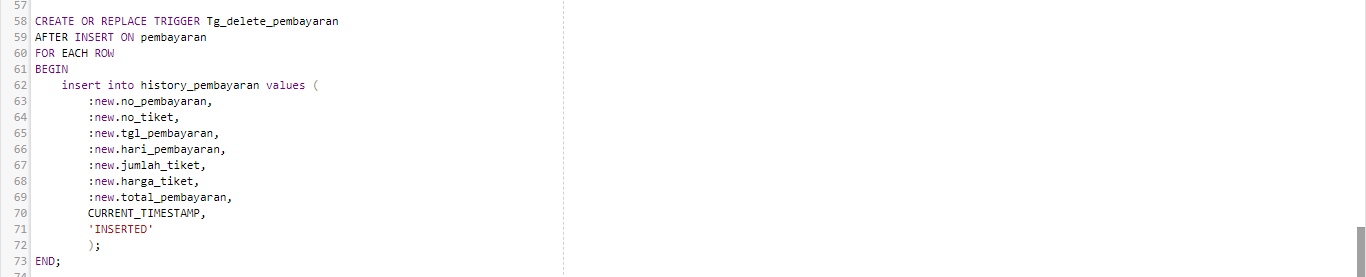
\includegraphics[width=10cm]{insert.png}
    \end{center}
    View adalah perintah query yang disimpan pada database dengan suatu nama tertentu, sehingga bisa digunakan setiap saat untuk melihat data tanpa menuliskan ulang query tersebut.
    Kegunaan View:
    tujuan dari pembuatan VIEW adalah untuk kenyamanan (mempermudah penulisan query), untuk keamanan (menyembunyikan beberapa kolom yang bersifat rahasia), atau dalam beberapa kasus bisa digunakan untuk mempercepat proses menampilkan data (terutama jika kita akan menjalankan query tersebut secara berulang).
    \end{enumerate}

\section{Langkah-Langkah Membuat Aplikasi Oracle APEX}
\begin{enumerate}
    \item Setelah selesai membuat persiapan, maka langakah selanjutnya membuat aplikasi
    \item pilih app builder kemudian pilih create terlebih dahulu untuk membuat aplikasinya.
    \begin{center}
    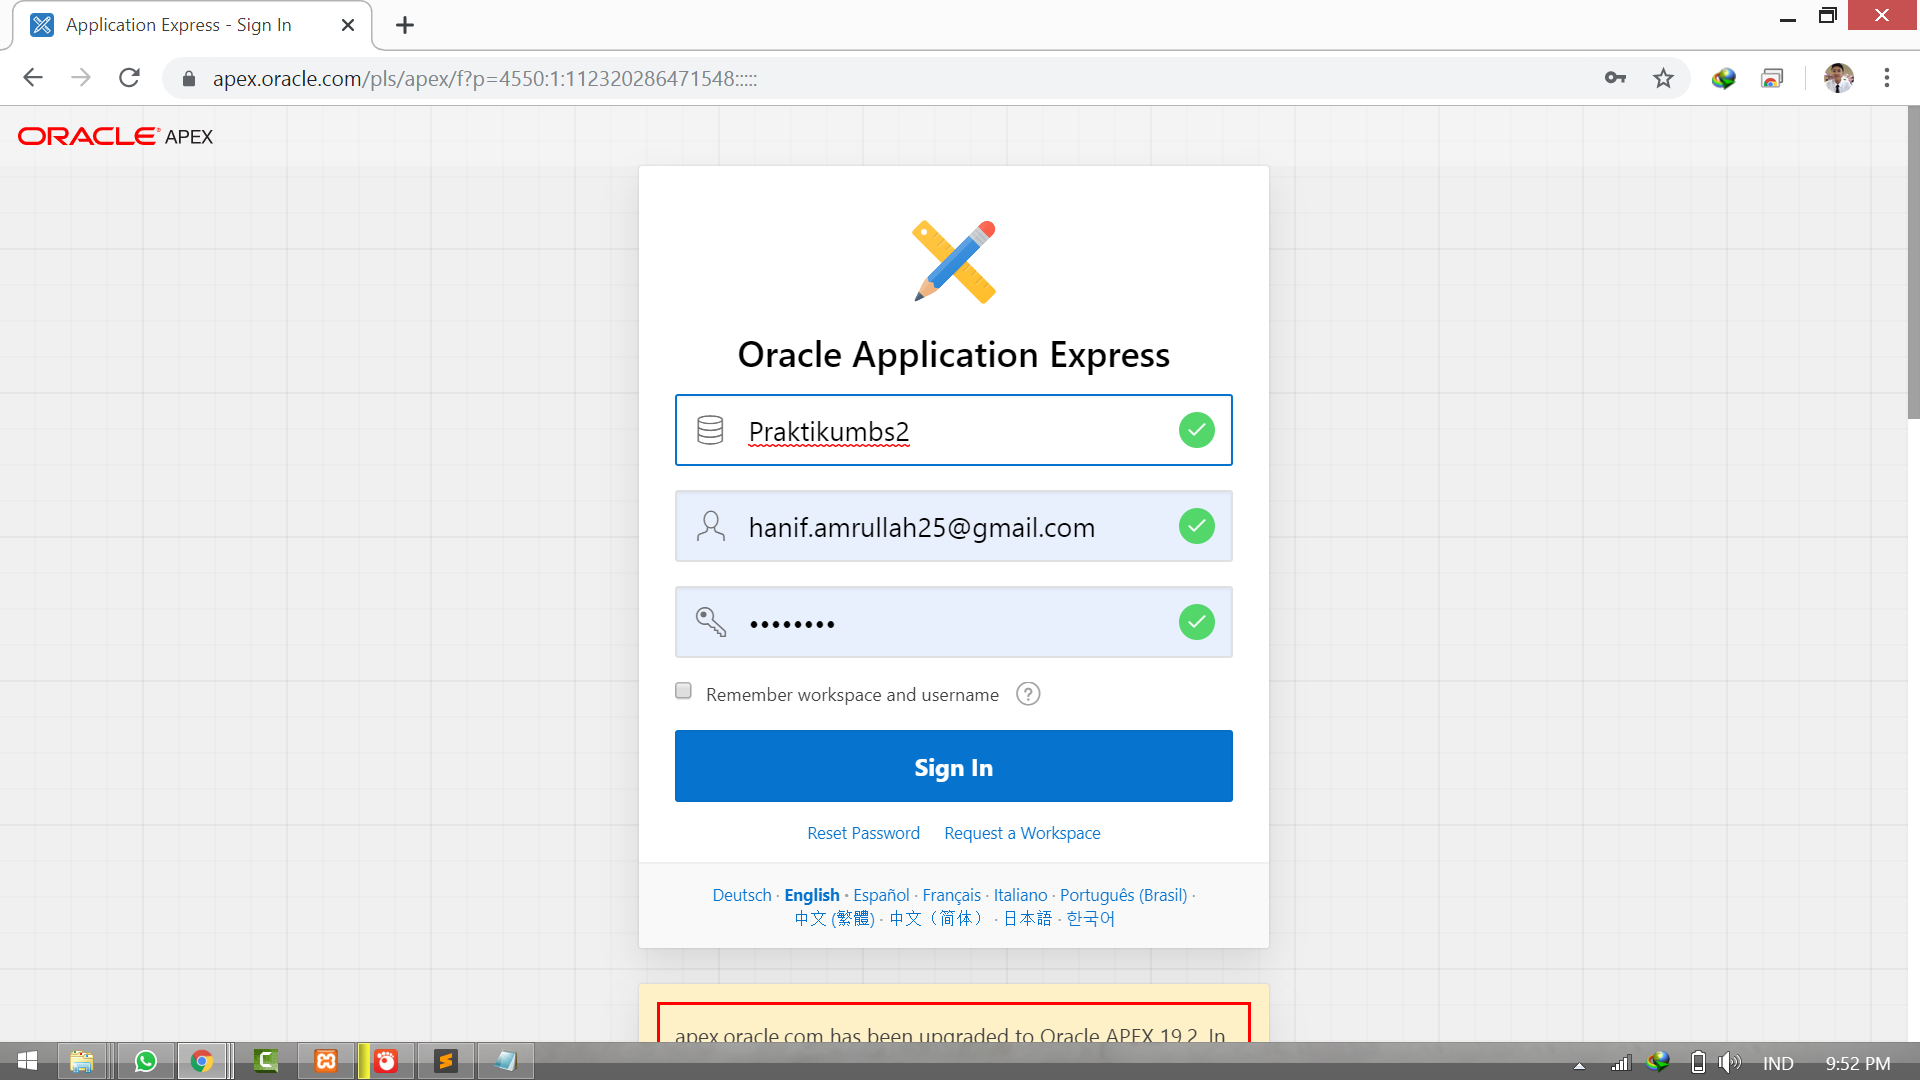
\includegraphics[width=10cm]{1.png}
    \end{center}
    \item lalu pilih new application 
    \begin{center}
    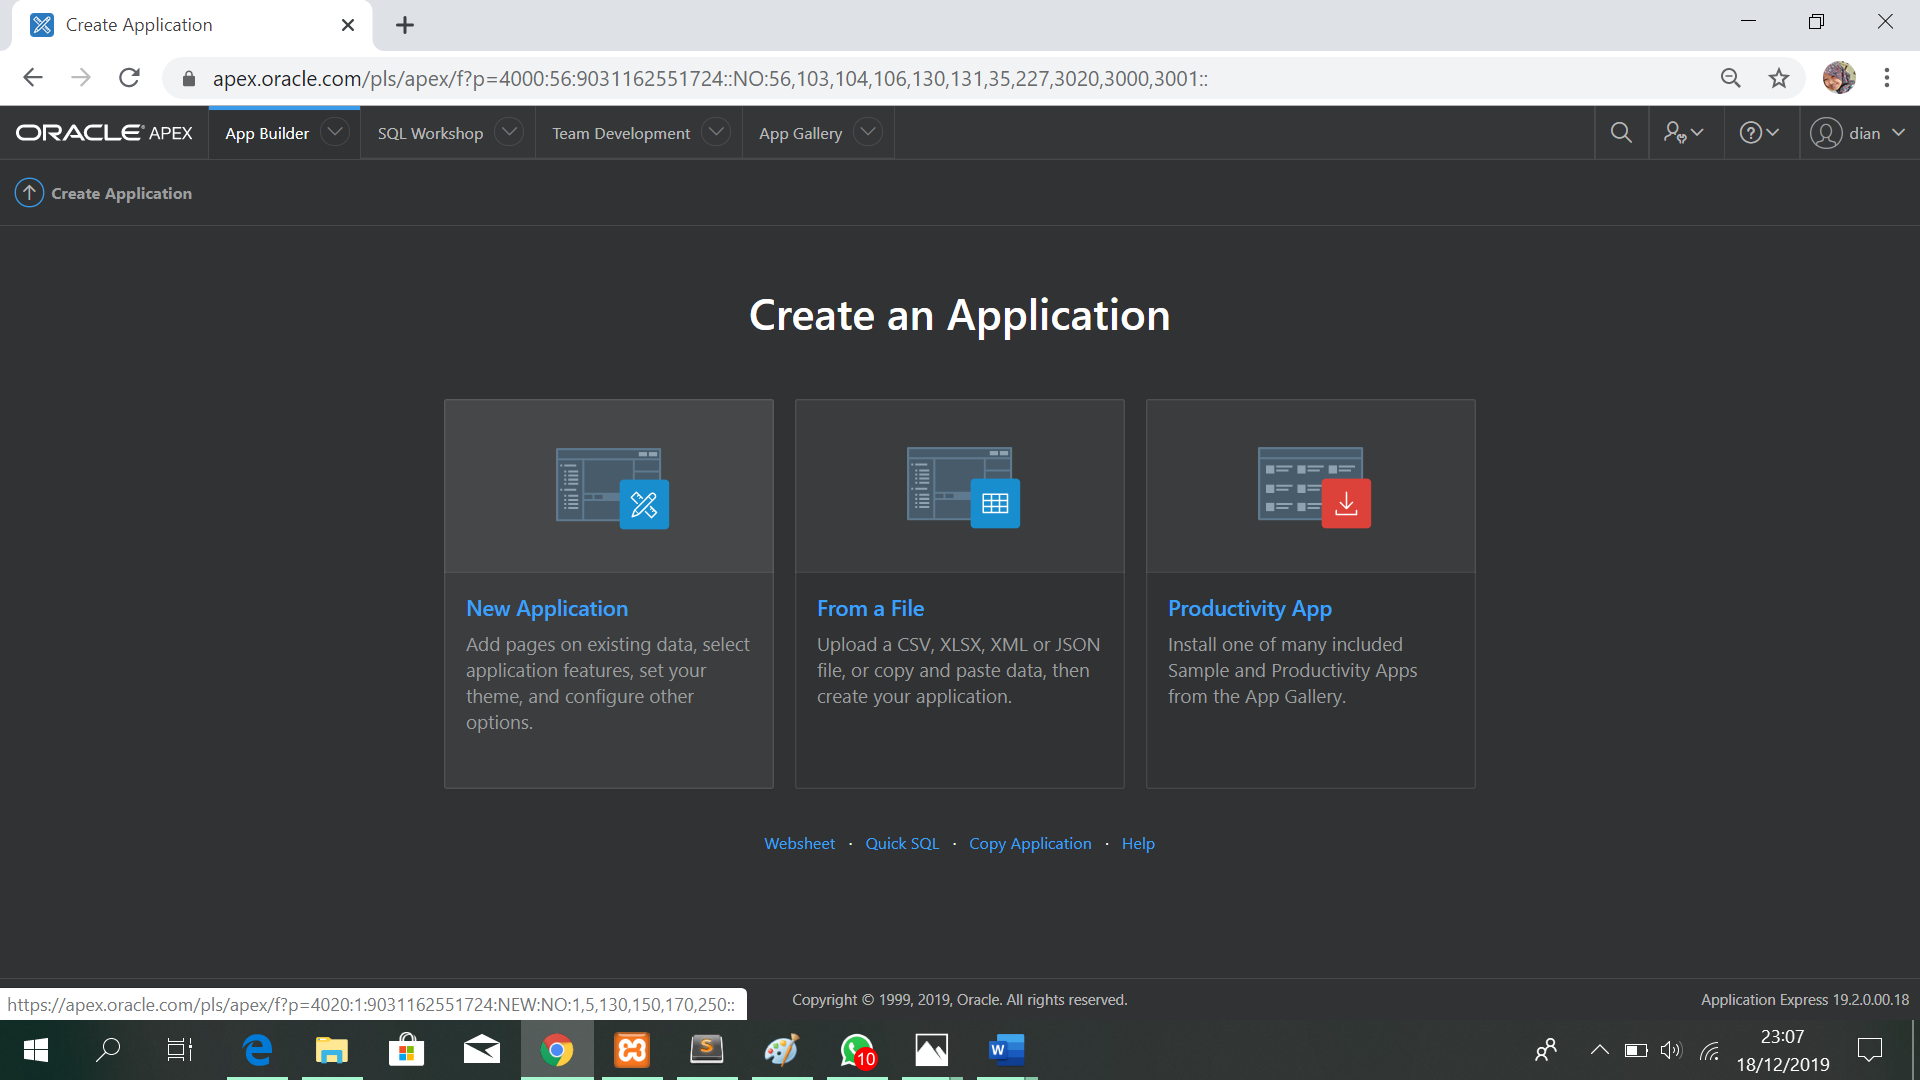
\includegraphics[width=10cm]{2.png}
    \end{center}
    \item Beri nama aplikasi yang akan kita buat 
    \begin{center}
    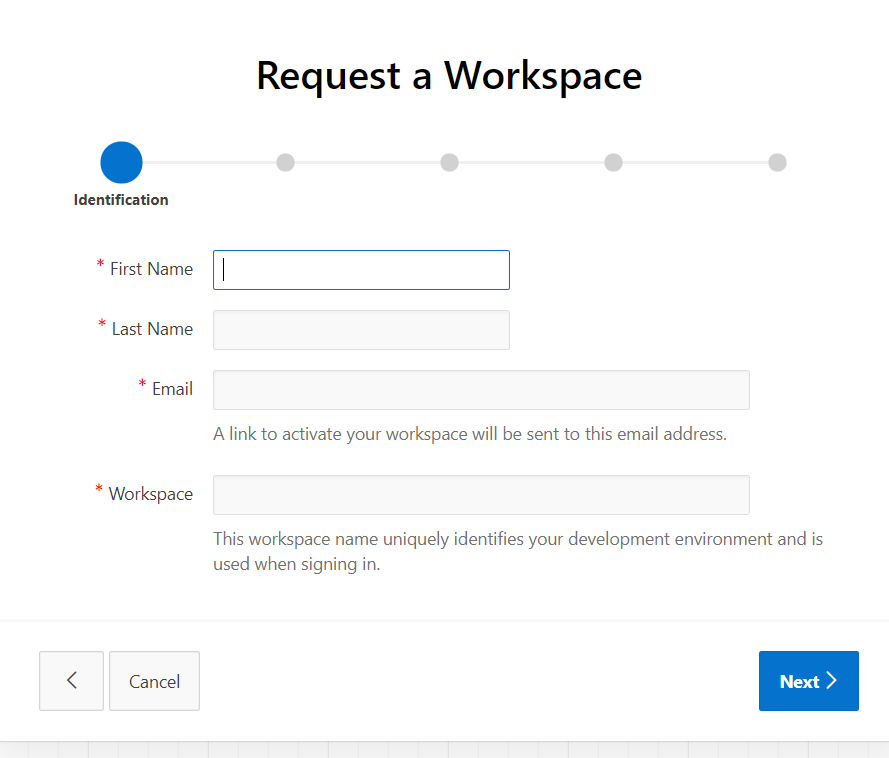
\includegraphics[width=10cm]{3.png}
    \end{center}
    \item pilih add page sesuai dengan tablenya, seperti table konsumen
    \begin{center}
    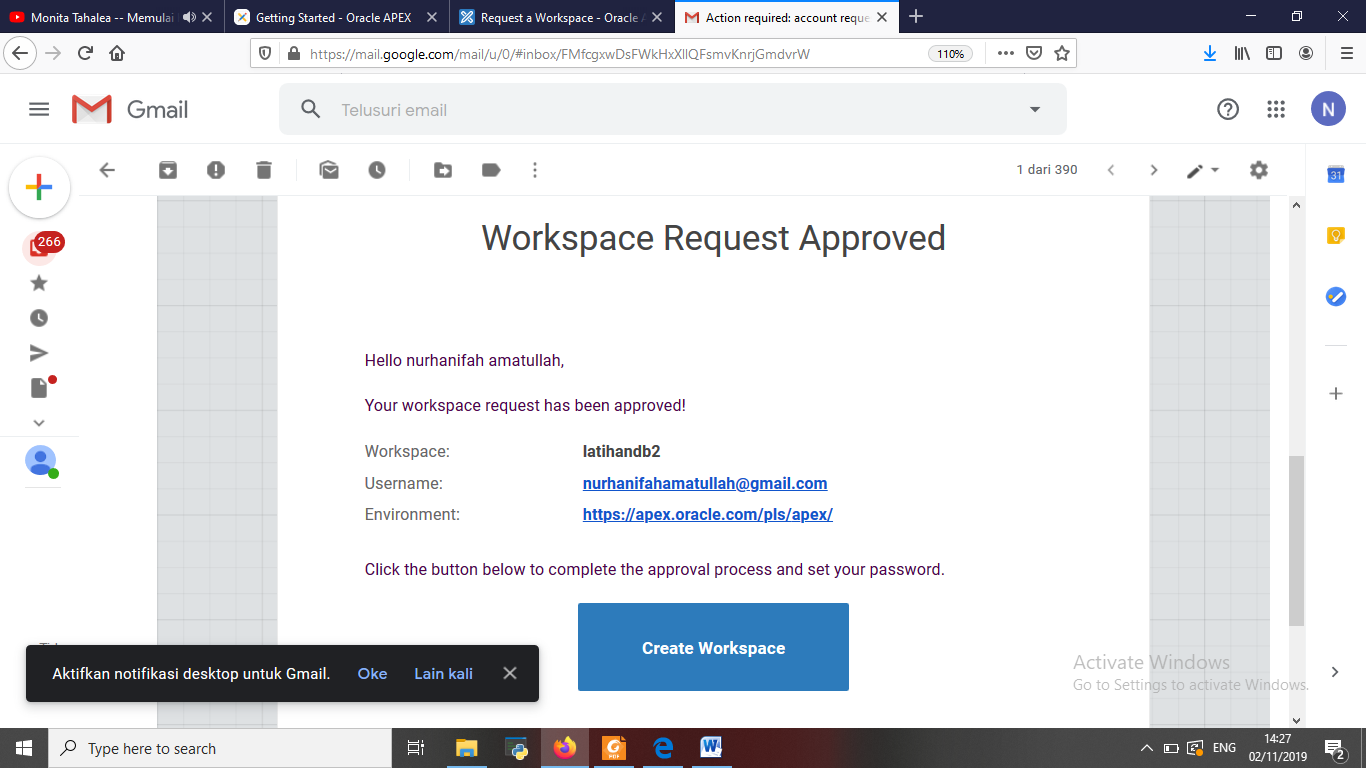
\includegraphics[width=10cm]{6.png}
    \end{center}
    Begitupun pada table berikutnya untuk menambahkan add page yang sesuai dengan tampilan table yang akan diinginkan.
    \item Jangan lupa untuk menceklis "check all"
    \begin{center}
    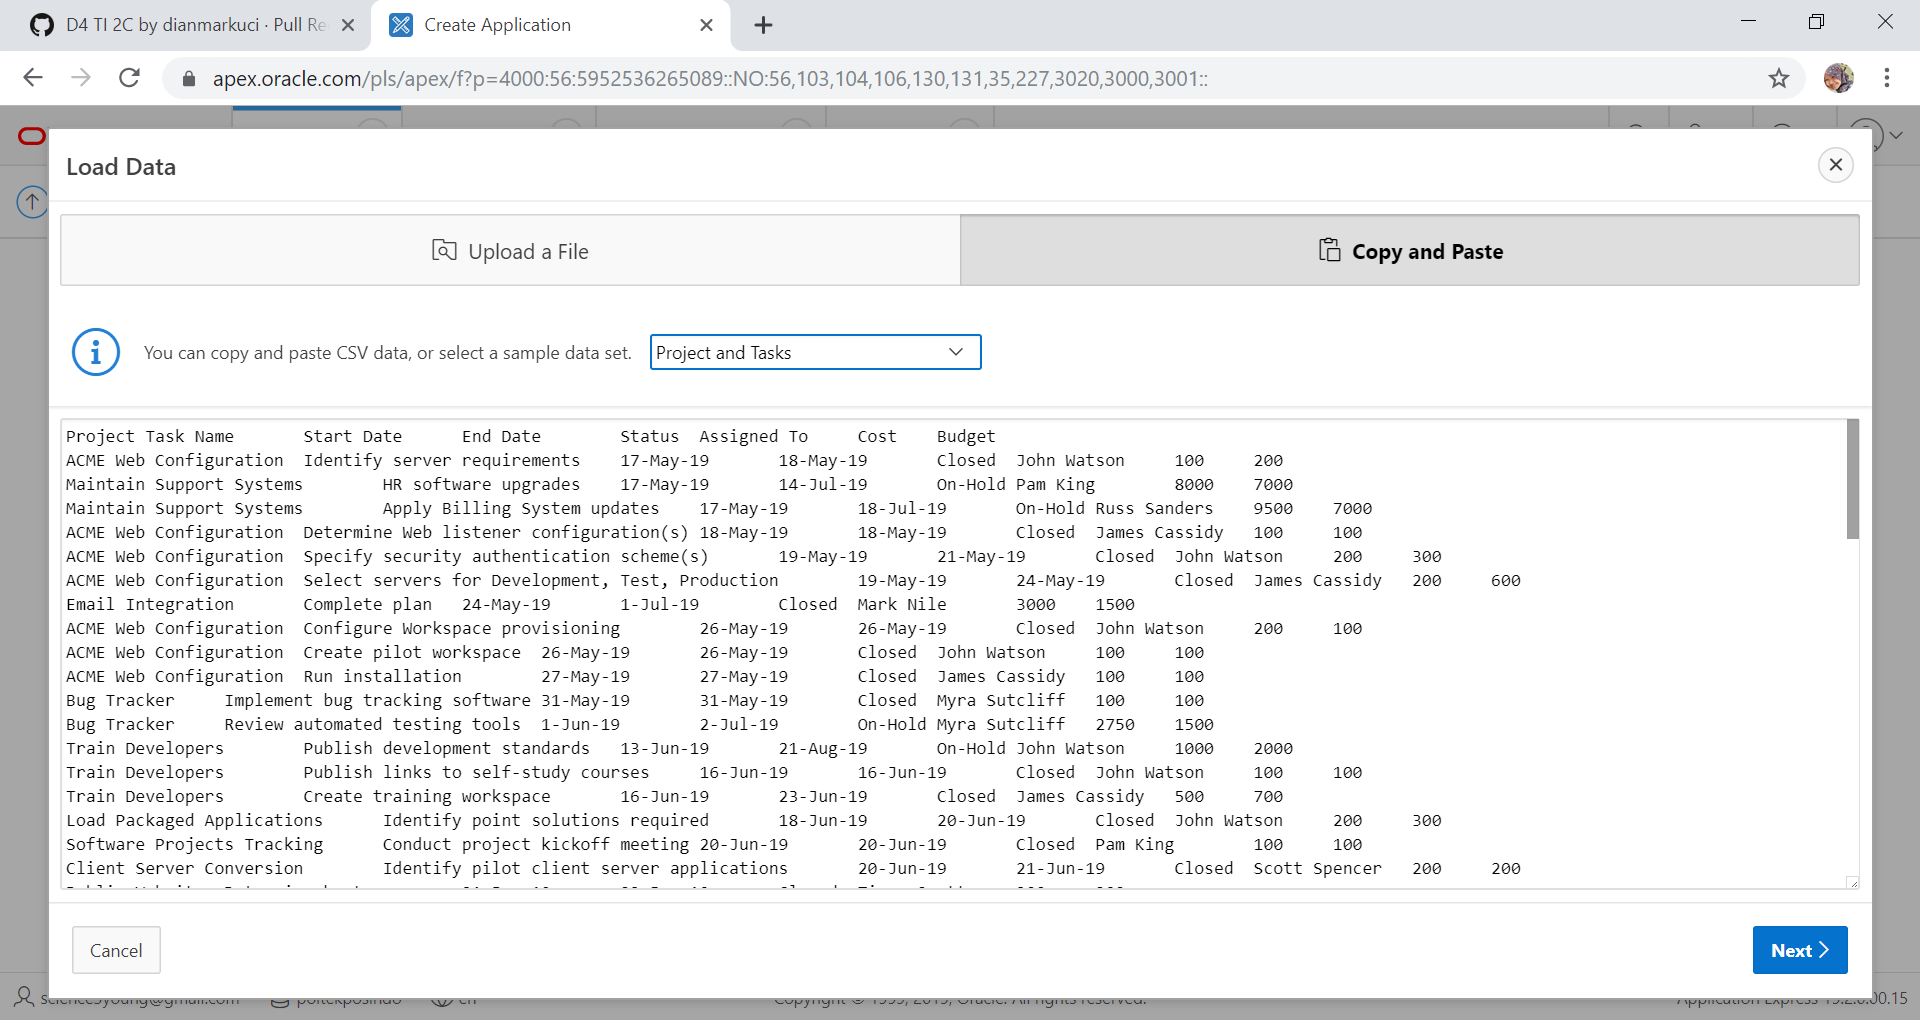
\includegraphics[width=10cm]{7.png}
    \end{center}
    \item Lalu pilih create application, dan tunggu loadingnya.
    \begin{center}
    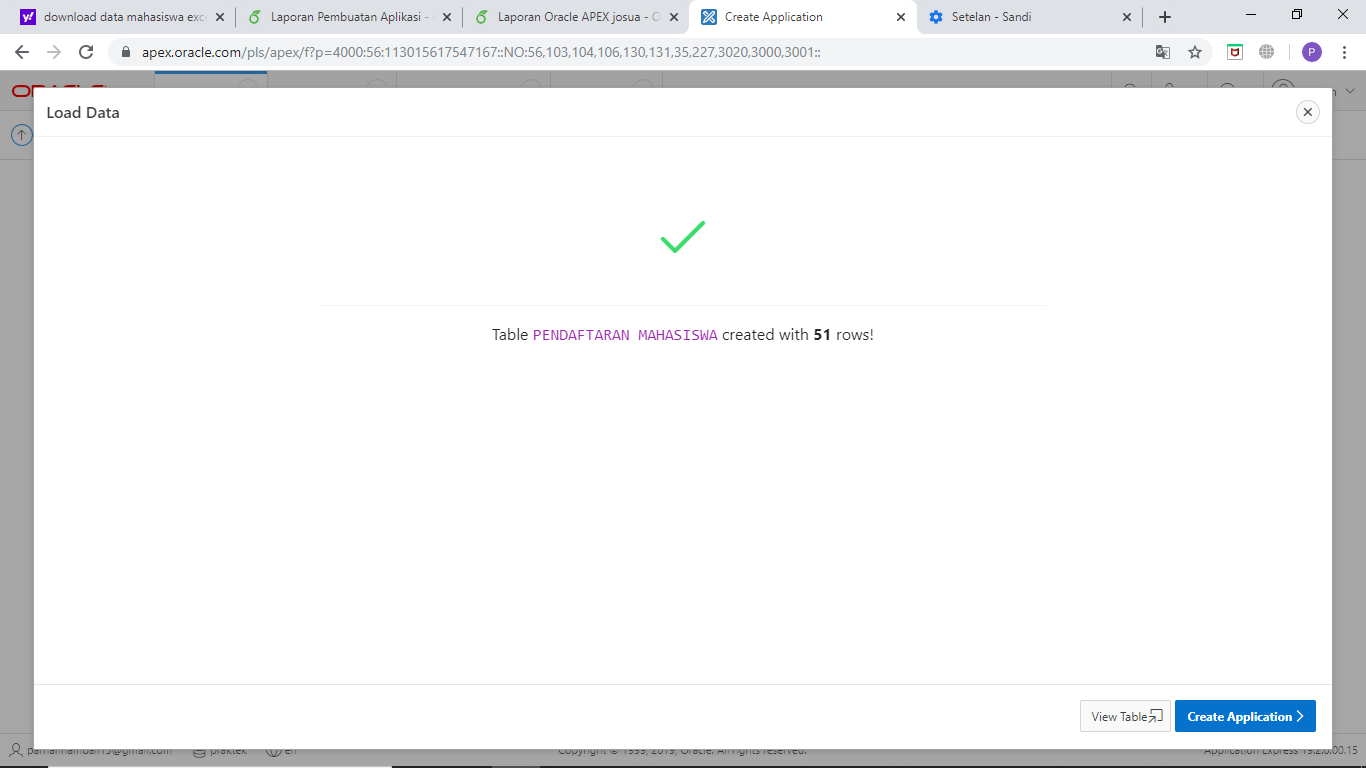
\includegraphics[width=10cm]{8.png}
    \end{center}
    \item Kemudian Run Application
    \begin{center}
    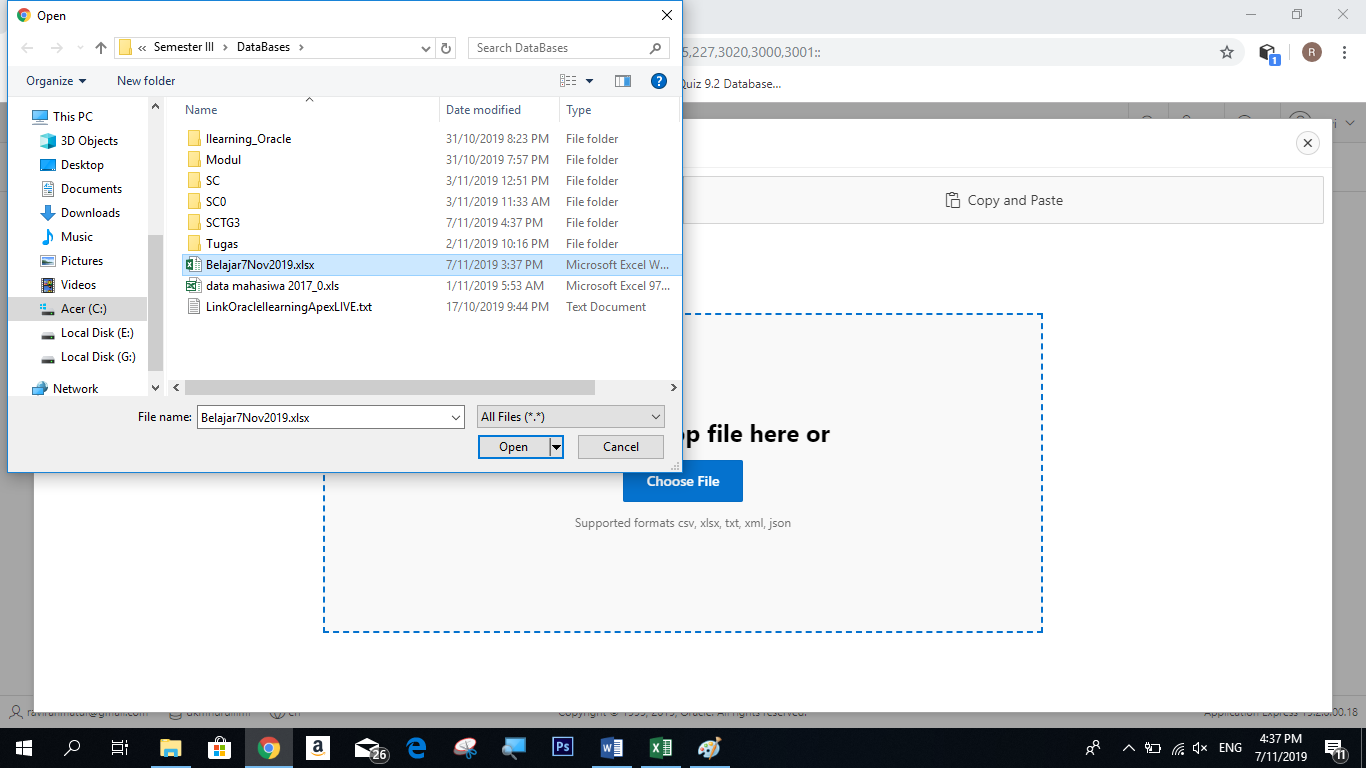
\includegraphics[width=10cm]{9.png}
    \end{center}
    \item Dan akhirnya aplikasi sudah jadi, di bawah ini merupakan tampilan halaman utama.
    \begin{center}
    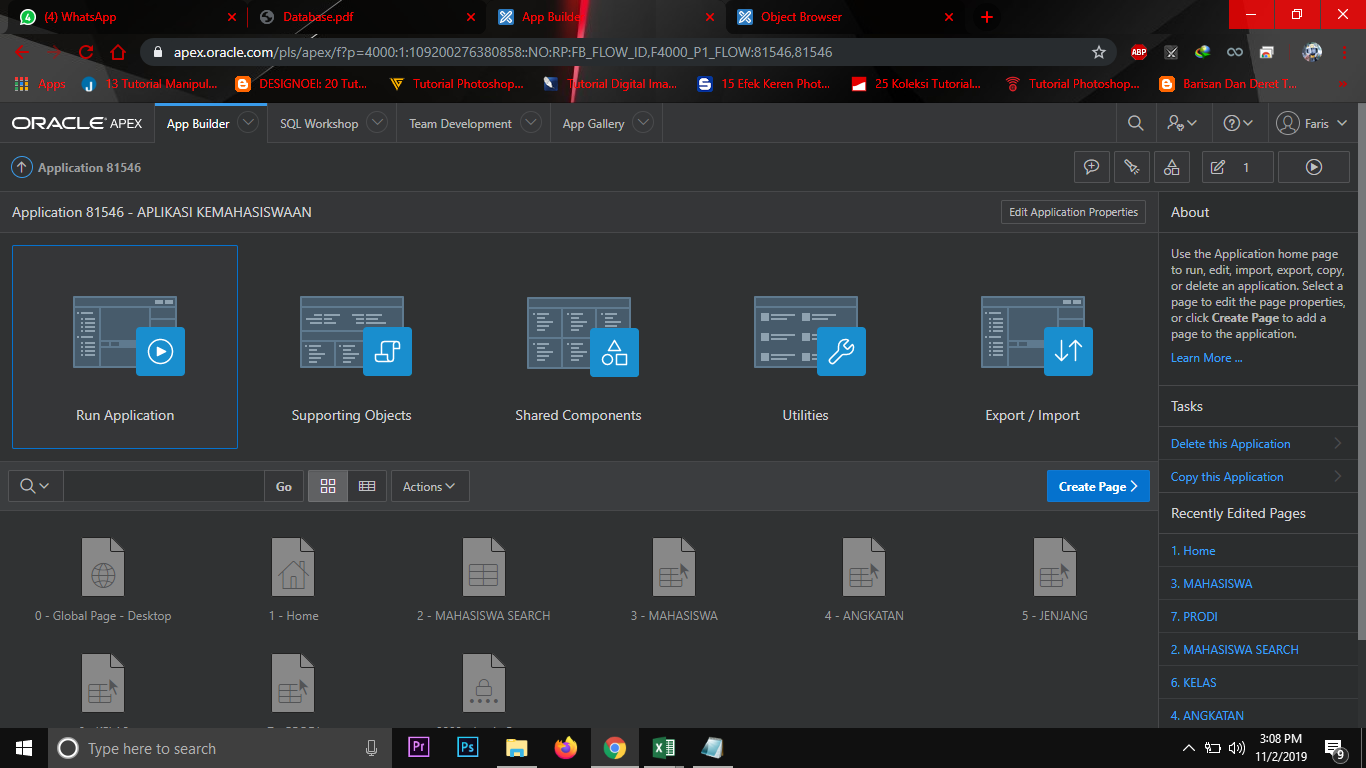
\includegraphics[width=10cm]{11.png}
    \end{center}
    \item Namun sebelum tampil ke halaman utama harus login terlebih dahulu, dengan membuka web browser dengan linknya https://apex.oracle.com/pls/apex/f?p=70668:LOGIN_DESKTOP:704904430066013:::::, kemudian menginputkan username:AYUANANDRA4@GMAIL.COM, password:anandra4, dan 
    
\end{enumerate}




\end{document}
